%==============================================================================
% Sjabloon poster bachproef
%==============================================================================
% Gebaseerd op document class `a0poster' door Gerlinde Kettl en Matthias Weiser
% Aangepast voor gebruik aan HOGENT door Jens Buysse en Bert Van Vreckem

\documentclass[a0,portrait]{hogent-poster}


% Info over de opleiding
\course{Bachelorproef}
\studyprogramme{toegepaste informatica}
\academicyear{2022-2023}
\institution{Hogeschool Gent, Valentin Vaerwyckweg 1, 9000 Gent}

% Info over de bachelorproef
\title{\Huge Scholieren met dyslexie van de derde graad middelbaar onderwijs ondersteunen bij het begrijpend lezen van wetenschappelijke artikelen via gepersonaliseerde ATS.}

\subtitle{}
\author{Dylan Cluyse}
\email{dylan.cluyse@student.hogent.be}
\supervisor{Lena De Mol}
\cosupervisor{Johan Decorte (Hogeschool Gent); Jana Van Damme (Hogeschool Gent)}

% Indien ingevuld, wordt deze informatie toegevoegd aan het einde van de
% abstract. Zet in commentaar als je dit niet wilt.
\specialisation{AI en data engineering}
\keywords{Gepersonaliseerde tekstvereenvoudiging; dyslexie; natuurlijke taalverwerking}
\projectrepo{https://github.com/dylancluyse/bachelorproef-nlp-tekstvereenvoudiging}

\begin{document}

\maketitle

\begin{abstract}
Ingewikkelde woordenschat en zinsbouw hinderen scholieren met dyslexie in de derde graad van het middelbaar onderwijs bij het begrijpend lezen van wetenschappelijke artikelen. Gepersonaliseerde \textit{manual text simplification} (MTS) helpt deze scholieren bij het begrijpend lezen. Daarnaast kan \textit{automatic text simplification} (ATS) dit proces automatiseren om de werkdruk bij leraren en scholieren te verminderen. Dit onderzoek achterhaalt met welke technologische en logopedische aspecten AI-ontwikkelaars rekening moeten houden bij de ontwikkeling van een AI-toepassing voor geautomatiseerde en gepersonaliseerde tekstvereenvoudiging. Hiervoor stelt het onderzoek de volgende onderzoeksvraag op: "Hoe kan een machine een wetenschappelijk artikel automatisch vereenvoudigen op maat van de noden van scholieren met dyslexie in de derde graad middelbaar onderwijs?". Een requirementsanalyse achterhaalt de nodige functionaliteiten om gepersonaliseerde ATS mogelijk te maken. Vervolgens vergelijkt het onderzoek bestaande \textit{pre-trained} taalmodellen om te zien welk taalmodel ontwikkelaars kunnen inzetten om de taak van gepersonaliseerde ATS mogelijk te maken. De requirementsanalyse wijst uit dat ontwikkelaars de geteste toepassingen voor een centrale doelgroep ontwikkelen en daarmee geen rekening houden met de noden van een scholier met dyslexie in de derde graad middelbaar onderwijs. Toepassingen voor gepersonaliseerde ATS zijn mogelijk, maar ontwikkelaars moeten meer inzetten op de noden van deze scholieren.
\end{abstract}

\begin{multicols}{2} % This is how many columns your poster will be broken into, a portrait poster is generally split into 2 columns

\section{Introductie}

% Zin uit script nemen --> in inleiding
% 'vindt u deze zin moeilijk om te lezen'


% Tweede filmpje bekijken
% voor- en na
% cumuleerbare

\begin{quotation}
\textit{Tsageinpoesn voor glesriaenseperode ATS zijn mejligok, maar okaweilnktras mteeon meer itetzenn op de ukinee ndoen van deze sielchreon.}
\end{quotation}

Vindt u deze zin moeilijk te lezen? Dit kan voor scholieren met dyslexie dagelijkse kost zijn bij het begrijpend lezen. Daarnaast kan het vakjargon en een compact formaat het begrijpend lezen van nieuw wetenschappelijk onderzoek hinderen. Toch kunnen leerkrachten deze obstakels verwijderen voor scholieren met \textit{manual text simplification} (MTS). Om de werkdruk in het onderwijs tegen te gaan, moeten systemen dit proces automatiseren met \textit{automated text simplification} (ATS). Dit onderzoek bekijkt hoe ontwikkelaars dergelijk toepassingen voor gepersonaliseerde ATS voor wetenschappelijke artikelen kunnen ontwikkelen. Figuur \ref{img:onderzoeksvragen} toont de centrale onderzoeksvraag samen met de nodige deelvragen. Zo kan dit onderzoek zowel leerkrachten als alle scholieren (met/zonder dyslexie) baten.

\begin{center}
	\captionsetup{type=figure}
	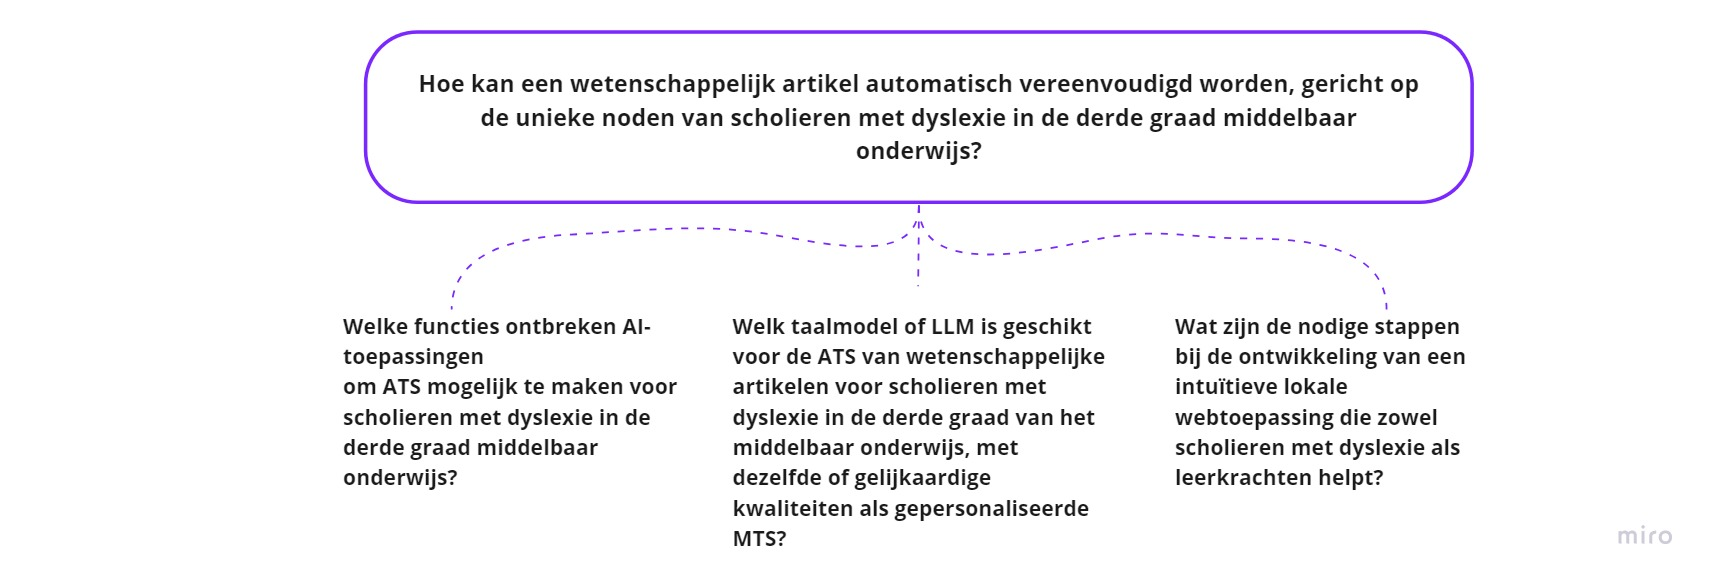
\includegraphics[width=1.0\linewidth]{figures/onderzoeksvragen.jpg}
	\captionof{figure}{Centraal de onderzoeksvraag met daaronder drie deelvragen die het onderzoek moet kunnen beantwoorden.}
	\label{img:onderzoeksvragen}
\end{center}

\section{Onderzoeksmethoden}

Om een werkwijze te achterhalen voor het ontwikkelen van dergelijk toepassing, voert het onderzoek drie fasen uit weergegeven op figuur \ref{img:flowchart}. Allereerst toetst de requirementsanalyse de huidige toepassingen af op hun MTS-functionaliteiten met een moscow-schema. Daarna vergelijkt het onderzoek beschikbare taalmodellen met machinale en menselijke beoordeling. Machinale scores gebeuren met python-scripts die leesbaarheidsscores per zin genereren. Daarnaast dienen MTS-referentieteksten van leerkrachten en scholieren als spreekwoordelijke spiegel voor ATS-teksten om gelijkenissen en ontbrekende technieken te achterhalen. Tot slot bouwt het onderzoek een prototype op waarin alle \textit{must-have} MTS-technieken aan bod moeten komen. Het prototype bestaat uit twee componenten, namelijk een scholieren- en een lerarencomponent.

\begin{center}
	\captionsetup{type=figure}
	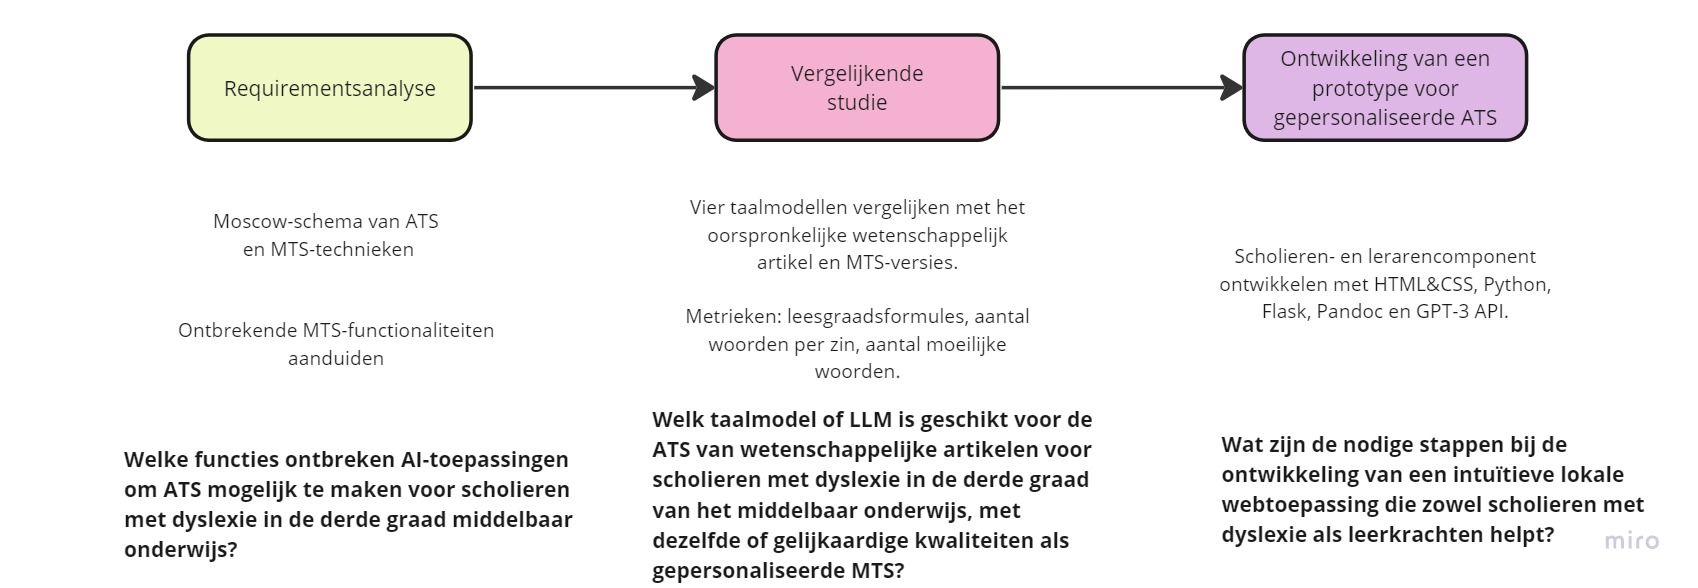
\includegraphics[width=1.0\linewidth]{figures/onderzoeksmethoden.jpg}
	\captionof{figure}{De gebruikte onderzoeksmethoden. In het vetgedrukt staan de onderzoeksvragen beschreven.}
	\label{img:flowchart}
\end{center}

\section{Resultaten}

% requirementsanalyse
Uit de requirementsanalyse blijkt dat bestaande online tools en softwaretoepassingen voor ATS onvoldoende gepersonaliseerde functionaliteiten bieden. Ze ontbreken opmaakopties voor scholieren met dyslexie. Recente technologieën bieden wel tekstvereenvoudigingsopties, maar vereisen informaticakennis die scholieren en leraren niet kunnen hebben. Taalmodellen T1, T2 en T3 maken ATS-teksten die geen rekening houden met de doelgroep. Daarnaast blijft het aantal lange en ingewikkelde woorden boven dat van de MTS-teksten en het oorspronkelijk wetenschappelijk artikel, zoals aangegeven in figuur \ref{img:results}. T4 slaagt er wel in om zinnen te maken die eenvoudiger zijn dan de oorspronkelijke tekst en kan personaliseerbare uitvoer maken. Beide componenten beschikken over alle \textit{must-have} technieken. Zo kunnen scholieren tekst in een personaliseerbare weergave van het oorspronkelijke artikel vereenvoudigen met alle MTS-technieken. Daarnaast kunnen leerkrachten een gepersonaliseerde ATS van een wetenschappelijk artikel in pdf of docx-formaat laten maken met het prototype.

\begin{center}
	\captionsetup{type=figure}
	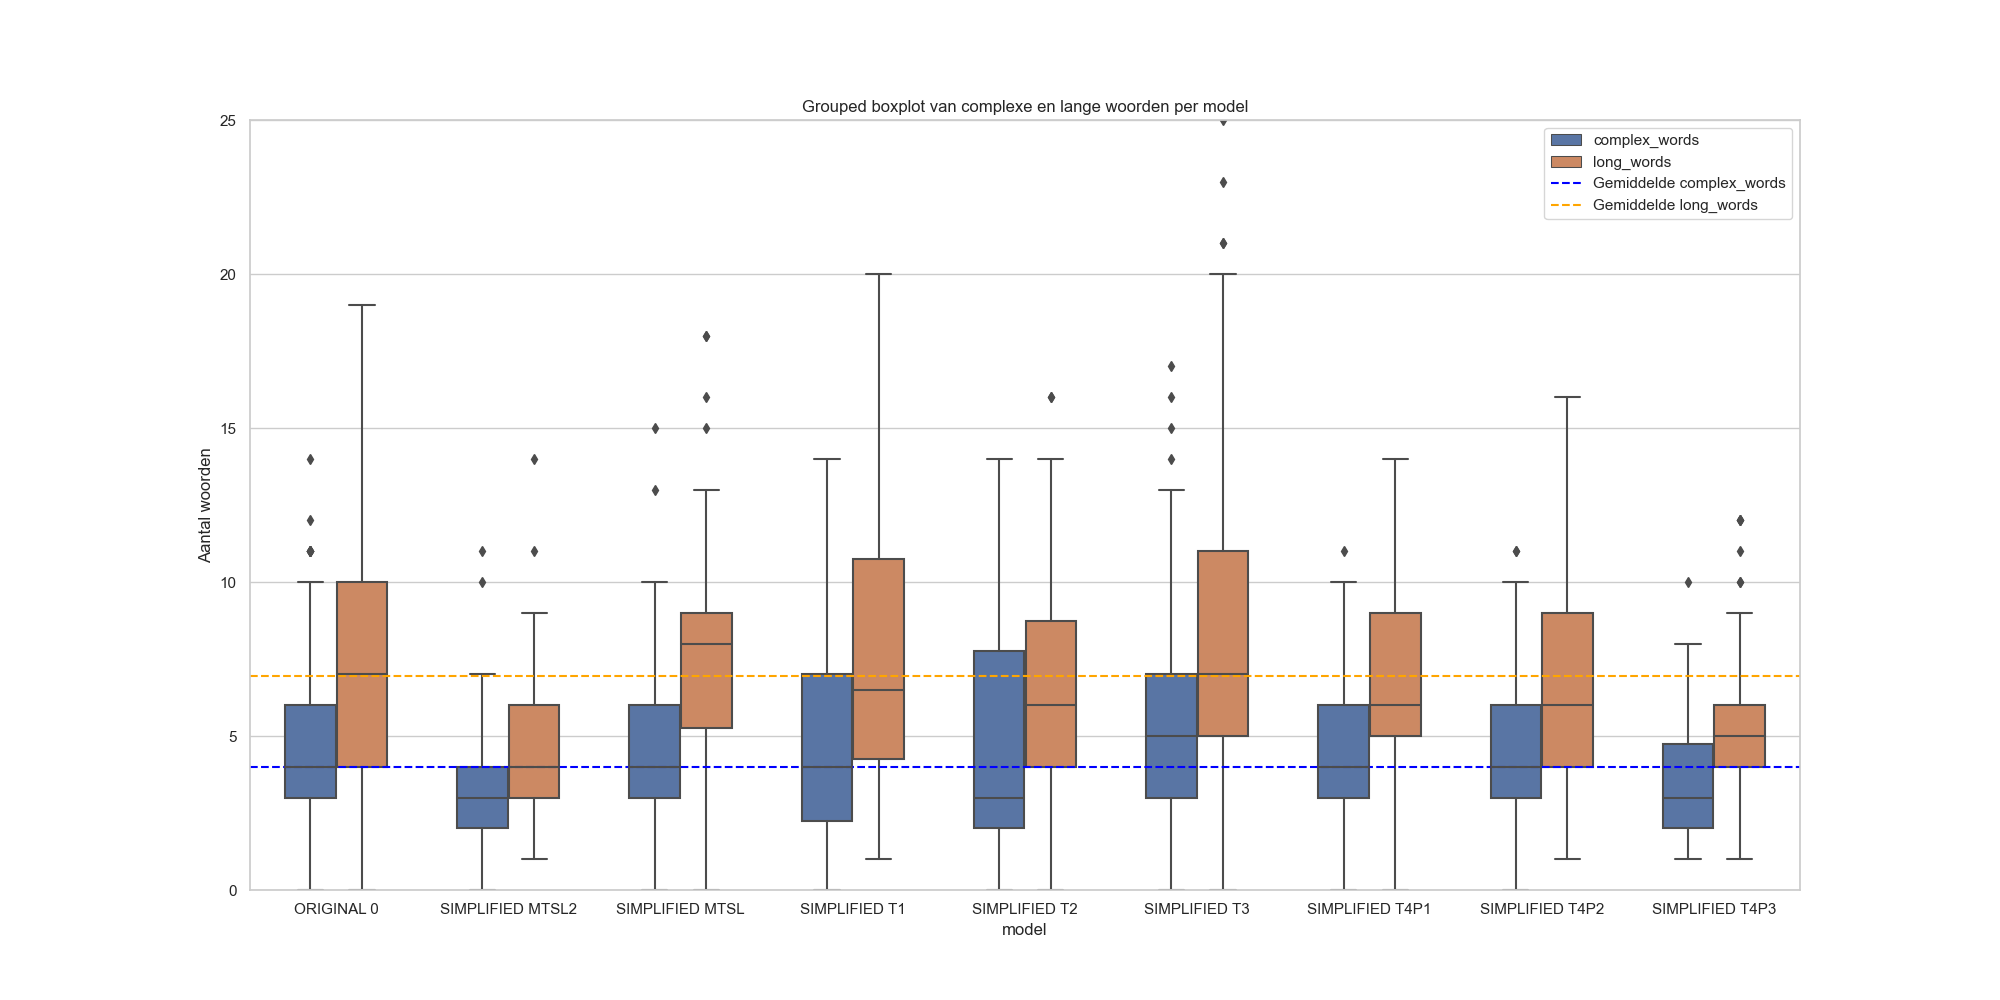
\includegraphics[width=1.0\linewidth]{figures/boxplot-poster.png}
	\captionof{figure}{De machinale beoordeling van de vereenvoudigde teksten.}
	\label{img:results}
\end{center}

%Alle onderzochte MTS-technieken, buiten actief naar passief schrijven en het verwerken van signaalwoorden, komen bij GPT-3 aan bod. 

\section{Conclusies}
Huidige toepassingen ontbreken de nodige MTS-technieken om gepersonaliseerde ATS aan te reiken of bieden deze aan in de vorm van prompts. Promptgebaseerde toepassingen zijn personaliseerbaar en daarmee geschikte taalmodellen voor de vereenvoudiging van wetenschappelijke artikelen voor scholieren met dyslexie. Hoewel het prototype niet alle \textit{should-have} en \textit{could-have} functionaliteiten beschikken, kunnen ontwikkelaars met de gebruikte softwarepakketten een volledig afgewerkte toepassing ontwikkelen.

% onderzoeksvraag
Om een systeem voor gepersonaliseerde ATS van voor scholieren met dyslexie in de derde graad van het middelbaar onderwijs te ontwikkelen, moeten ontwikkelaars rekening houden met het gekozen taalmodel en de opgenomen MTS-functionaliteiten. GPT-3 vergt nog experimentatie, maar kan optreden als bouwsteen voor gepersonaliseerde ATS. Tot slot toont figuur \ref{img:verder-onderzoek} aspecten waarop onderzoekers van dit onderzoek kunnen verderdoen. Zo kunnen toekomstige onderzoeken experimenten uitvoeren met dit prototype, dankzij de eenduidige opzet met Docker en scriptbestanden.

\begin{center}
	\captionsetup{type=figure}
	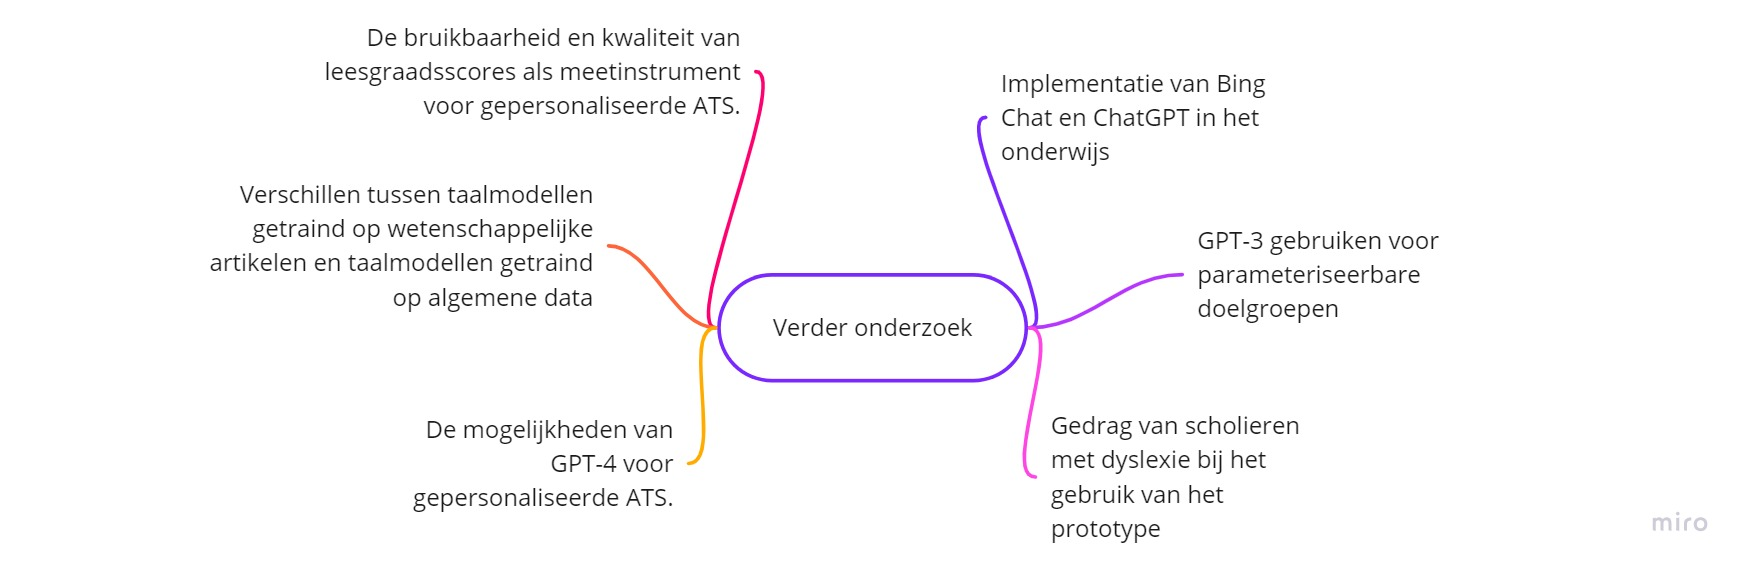
\includegraphics[width=1.0\linewidth]{figures/verder-onderzoek.jpg}
	\captionof{figure}{Onderzoeksonderwerpen die verder onderzoek vereisen.}
	\label{img:verder-onderzoek}
\end{center}

\end{multicols}
\end{document}